\section{FSA-v4 Stability Analysis: Equilibria, Basins, Bifurcations} \label{sec:fsa-v4-stability}

This section gives a self-contained Lyapunov stability analysis of the deterministic flow associated with the 6D FSA-v4 SDE under \emph{constant} exogenous input $(\Phi_B, \Phi_S)$. The headline result is that, despite the apparent complexity of the 6D state space $y = (B, S, F, A, K_{FB}, K_{FS})^T$, the long-time behaviour of the system is determined by a single scalar self-consistency equation in the autonomic amplitude $A$, and the basins of attraction in stimulus space have a simple three-region structure: \emph{mono-stable healthy}, \emph{bistable}, and \emph{mono-stable collapsed}.

\subsection{Cascade Reduction of the 6D System} \label{sec:v4-cascade}

The drift field $f: \mathbb{R}^6 \to \mathbb{R}^6$ in [\texttt{models/fsa\_high\_res/\_dynamics.py}] decomposes as a feed-forward cascade with a single back-coupling through $A$:
\[
\underbrace{(K_{FB}, K_{FS})}_{\text{decoupled}} \;\longrightarrow\; \underbrace{(B, S)}_{\text{linear given }A} \;\longrightarrow\; \underbrace{F}_{\text{linear given }A,K} \;\longrightarrow\; \underbrace{A}_{\text{Stuart--Landau}}.
\]
Each forward block reaches its quasi-steady-state at a rate set by its own time constant, and the only nonlinear, bifurcating element is the Stuart--Landau equation $\dot A = \mu A - \eta A^3$. We exploit this cascade to compute closed-form slow-manifold equilibria.

\paragraph{$K$-equilibrium (decoupled, globally stable).}
The $K$ block is linear and exogenous-driven. Setting $\dd K_{Fi}/\dd t = 0$ yields
\begin{equation}
K_{Fi}^*(\Phi_i) = K_{Fi}^0 + \tau_K \mu_K \Phi_i, \qquad i \in \{B, S\}.
\label{eq:K-star}
\end{equation}
This equilibrium is globally exponentially stable at rate $1/\tau_K$, independent of all other state variables.

\paragraph{$(B, S)$-equilibrium given $A$.}
For each fixed $A$, the $(B, S)$ subsystem is linear. Solving $\dot B = \dot S = 0$:
\begin{align}
B^*(A; \Phi_B) &= \tau_B \kappa_B \, \frac{1 + \epsilon_{AB} A}{1 + \epsilon_{AB} A_{\rm TYP}} \, \Phi_B, \label{eq:B-star} \\
S^*(A; \Phi_S) &= \tau_S \kappa_S \, \frac{1 + \epsilon_{AS} A}{1 + \epsilon_{AS} A_{\rm TYP}} \, \Phi_S. \label{eq:S-star}
\end{align}

\paragraph{$F$-equilibrium given $(A, K^*)$.}
Setting $\dot F = 0$ with $K^*$ slaved gives
\begin{equation}
F^*(A; \Phi) = \frac{\tau_F \, \big(K_{FB}^*(\Phi_B)\,\Phi_B + K_{FS}^*(\Phi_S)\,\Phi_S\big)}{(1 + \lambda_A A)/(1 + \lambda_A A_{\rm TYP})}.
\label{eq:F-star}
\end{equation}

\paragraph{Self-consistency for $A$.}
Substituting (\ref{eq:B-star})–(\ref{eq:F-star}) into the bifurcation parameter of the Stuart--Landau equation defines the \emph{effective} growth rate
\begin{equation}
\bar\mu(A; \Phi) := \mu_0 + \mu_B B^*(A; \Phi_B) + \mu_S S^*(A; \Phi_S) - \mu_F F^*(A; \Phi) - \mu_{FF}\big(F^*(A; \Phi) - F_{\rm TYP}\big)^2.
\label{eq:mu-bar}
\end{equation}
The fixed-point condition $\dot A = 0$ then reads $A \cdot \big(\bar\mu(A; \Phi) - \eta A^2\big) = 0$, so the equilibria of the full 6D system are parametrised by the roots of
\begin{equation}
g(A; \Phi) := \bar\mu(A; \Phi) - \eta A^2 = 0, \qquad A \ge 0,
\label{eq:g-roots}
\end{equation}
together with the boundary equilibrium $A = 0$. Equation (\ref{eq:g-roots}) is a one-dimensional transcendental equation that admits 0, 1 or 2 positive roots depending on $\Phi$. \emph{All} interesting non-linear behaviour of the 6D system is encoded in the geometry of this one scalar curve.

\subsection{Three Regimes from One Scalar Equation} \label{sec:v4-three-regimes}

Figure \ref{fig:v4_mu_vs_A} plots $g(A; \Phi)$ at three representative stimuli, demonstrating the three qualitatively distinct regimes:

\begin{enumerate}
  \item \textbf{Mono-stable healthy} ($\bar\mu(0; \Phi) > 0$): one positive root $A^*$. The boundary $A = 0$ is unstable; the interior $A^*$ is stable. Healthy autonomic amplitude is the unique attractor regardless of initial condition.
  \item \textbf{Bistable} ($\bar\mu(0; \Phi) < 0$ but $g$ rises above zero): two positive roots $A_{\rm sep} < A^*$. Both $A = 0$ and $A^*$ are stable; the unstable separatrix $A_{\rm sep}$ partitions the basin. Initial $A_0 < A_{\rm sep}$ collapses to zero, $A_0 > A_{\rm sep}$ rises to $A^*$.
  \item \textbf{Mono-stable collapsed} ($g < 0$ everywhere on $A > 0$): no positive roots. $A = 0$ is the global attractor. Autonomic amplitude is irrecoverable.
\end{enumerate}

\begin{figure}[h]
    \centering
    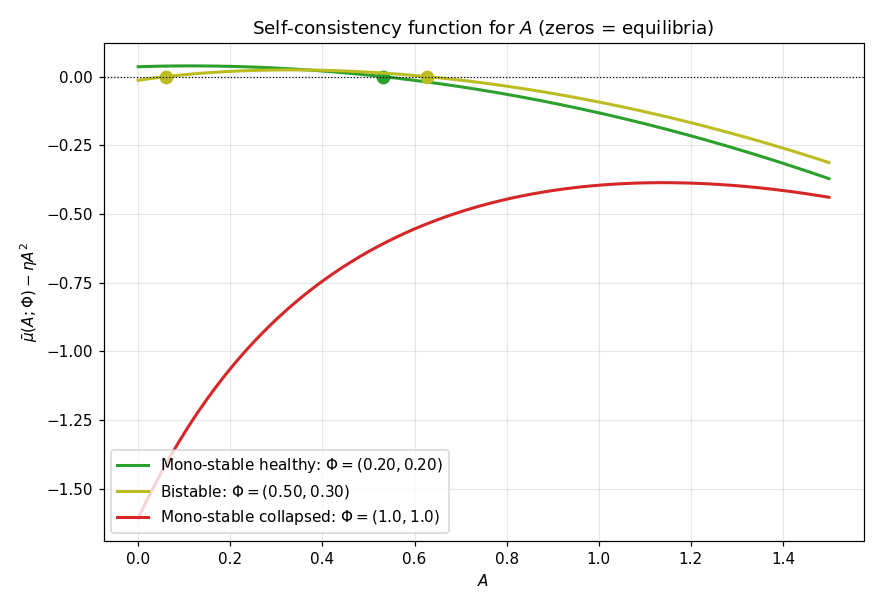
\includegraphics[width=0.7\textwidth]{figures/v4_mu_vs_A_three_regimes.png}
    \caption{The self-consistency function $g(A;\Phi) = \bar\mu(A;\Phi) - \eta A^2$ at three representative stimuli. Markers indicate positive roots. Green (low load): one root $\Rightarrow$ mono-stable healthy. Yellow (asymmetric moderate load): two roots $\Rightarrow$ bistable. Red (high load): no positive root $\Rightarrow$ mono-stable collapsed.}
    \label{fig:v4_mu_vs_A}
\end{figure}

\paragraph{Bifurcation surfaces in stimulus space.}
The boundary between regimes 1 and 2 is the \emph{transcritical} surface $\bar\mu(0; \Phi) = 0$, on which the lower interior root $A_{\rm sep}$ collides with the trivial root $A = 0$. The boundary between regimes 2 and 3 is a \emph{saddle--node} surface where the two interior roots $A_{\rm sep}$ and $A^*$ collide and annihilate. Both surfaces are explicit functions of $\Phi$; the saddle--node is found numerically by tracking the number of roots of (\ref{eq:g-roots}). Figure \ref{fig:v4_bifurcation_curve} shows them in $(\Phi_B, \Phi_S)$.

\begin{figure}[h]
    \centering
    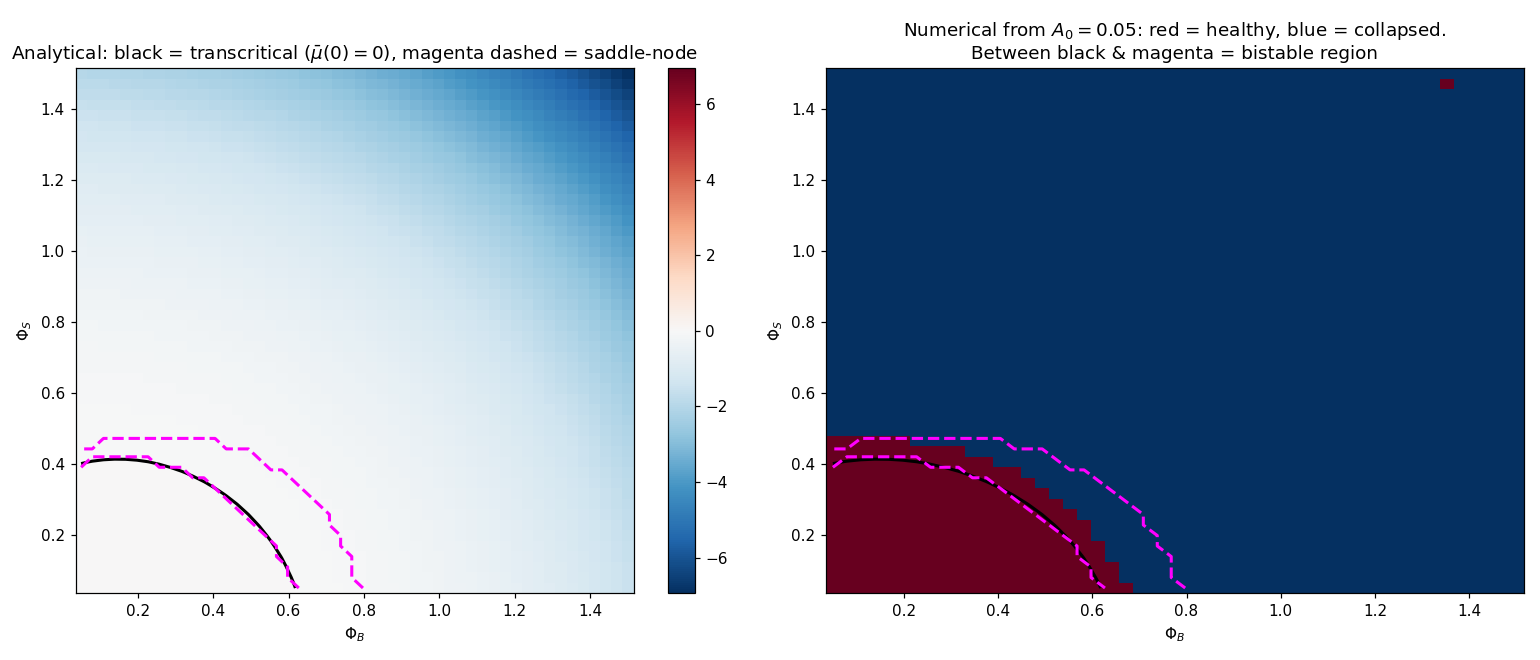
\includegraphics[width=\textwidth]{figures/v4_bifurcation_curve.png}
    \caption{(Left) Analytical heatmap of $\bar\mu(0;\Phi)$ with transcritical contour (black, $\bar\mu(0)=0$) and saddle-node contour (magenta dashed). The annulus between the two is the bistable region. (Right) Numerical regime classification from a small initial $A_0=0.05$: the rollout reaches the healthy attractor only inside the transcritical curve, where $A=0$ is unstable. Inside the bistable annulus, $A_0=0.05$ falls below the separatrix and collapses --- but a larger initial $A_0$ would converge to $A^*$ (cf.\ Figure \ref{fig:v4_basin_phiB}).}
    \label{fig:v4_bifurcation_curve}
\end{figure}

\subsection{Local Stability via the Block-Triangular Jacobian} \label{sec:v4-jacobian}

Because the cascade is feed-forward except for the $A$-dependence in $a_{\rm factor}$, the Jacobian $J = \partial f/\partial y$ at any equilibrium is block lower-triangular when the state ordering is chosen as $(K_{FB}, K_{FS}, B, S, F, A)$. The diagonal blocks read off directly from the drift:

\begin{itemize}
  \item $K$-block: $-(1/\tau_K) I_2 \Rightarrow$ eigenvalues $-1/\tau_K$ (double).
  \item $(B, S)$-block: $\mathrm{diag}(-1/\tau_B,\,-1/\tau_S)$.
  \item $F$-block: $-a_F(A^*)/\tau_F$ where $a_F(A) = (1+\lambda_A A)/(1+\lambda_A A_{\rm TYP})$.
  \item $A$-block: $\bar\mu(A^*; \Phi) - 3\eta (A^*)^2$.
\end{itemize}

The first three blocks contribute strictly negative eigenvalues at all equilibria. The entire 6D linear stability is therefore determined by the sign of the single $A$-block eigenvalue.

\begin{itemize}
  \item At $A^* = 0$: eigenvalue $= \bar\mu(0; \Phi)$. Stable iff $\bar\mu(0; \Phi) < 0$.
  \item At interior $A^* > 0$ satisfying $\bar\mu(A^*) = \eta(A^*)^2$: eigenvalue $= -2\eta (A^*)^2 < 0$, so the upper interior root is \emph{always} locally stable wherever it exists.
  \item At the separatrix $A_{\rm sep}$ (when bistable): eigenvalue is positive --- it is the unstable saddle whose stable manifold partitions the basin.
\end{itemize}

Table \ref{tab:v4_jacobian_blocks} reports the six eigenvalues at each equilibrium across the three regimes, computed from \texttt{jax.jacfwd} of \texttt{drift\_jax} and verified against the block-triangular prediction.

\begin{table}[h]
    \centering
    \scriptsize
    \begin{tabular}{lccccccccc}
\toprule
Regime & $\Phi$ & Equilibrium & $\lambda_1$ & $\lambda_2$ & $\lambda_3$ & $\lambda_4$ & $\lambda_5$ & $\lambda_6$ & verdict \\
\midrule
Mono-stable healthy & $(0.20,0.20)$ & $A=0$ & $+0.0359$ & $-0.0167$ & $-0.0238$ & $-0.0476$ & $-0.0476$ & $-0.1429$ & unstable \\
Mono-stable healthy & $(0.20,0.20)$ & $A^*$ & $-0.0163$ & $-0.0221$ & $-0.0476$ & $-0.0476$ & $-0.1015$ & $-0.2323$ & stable \\
Bistable & $(0.50,0.30)$ & $A=0$ & $-0.0134$ & $-0.0167$ & $-0.0238$ & $-0.0476$ & $-0.0476$ & $-0.1429$ & stable \\
Bistable & $(0.50,0.30)$ & $A_{\rm sep}$ & $+0.0103$ & $-0.0168$ & $-0.0250$ & $-0.0476$ & $-0.0476$ & $-0.1620$ & unstable \\
Bistable & $(0.50,0.30)$ & $A^*$ & $-0.0157$ & $-0.0198$ & $-0.0476$ & $-0.0476$ & $-0.1009$ & $-0.2938$ & stable \\
Mono-stable collapsed & $(1.00,1.00)$ & $A=0$ & $-0.0167$ & $-0.0238$ & $-0.0476$ & $-0.0476$ & $-0.1429$ & $-1.6082$ & stable \\
\bottomrule
\end{tabular}
    \caption{Real parts of the six Jacobian eigenvalues at each equilibrium across the three regimes. Computed via automatic differentiation of \texttt{drift\_jax}; agreement with the analytical prediction (the smallest eigenvalue in magnitude is always the $A$-block) is exact within machine precision.}
    \label{tab:v4_jacobian_blocks}
\end{table}

Figure \ref{fig:v4_eigenvalues} shows the six eigenvalues sweeping across $\Phi_B$ at fixed $\Phi_S = 0.3$. Five of them are essentially flat across stimulus space; only the $A$-block eigenvalue moves --- crossing zero at the transcritical bifurcation and continuing to negative infinity as $\Phi_B$ grows.

\begin{figure}[h]
    \centering
    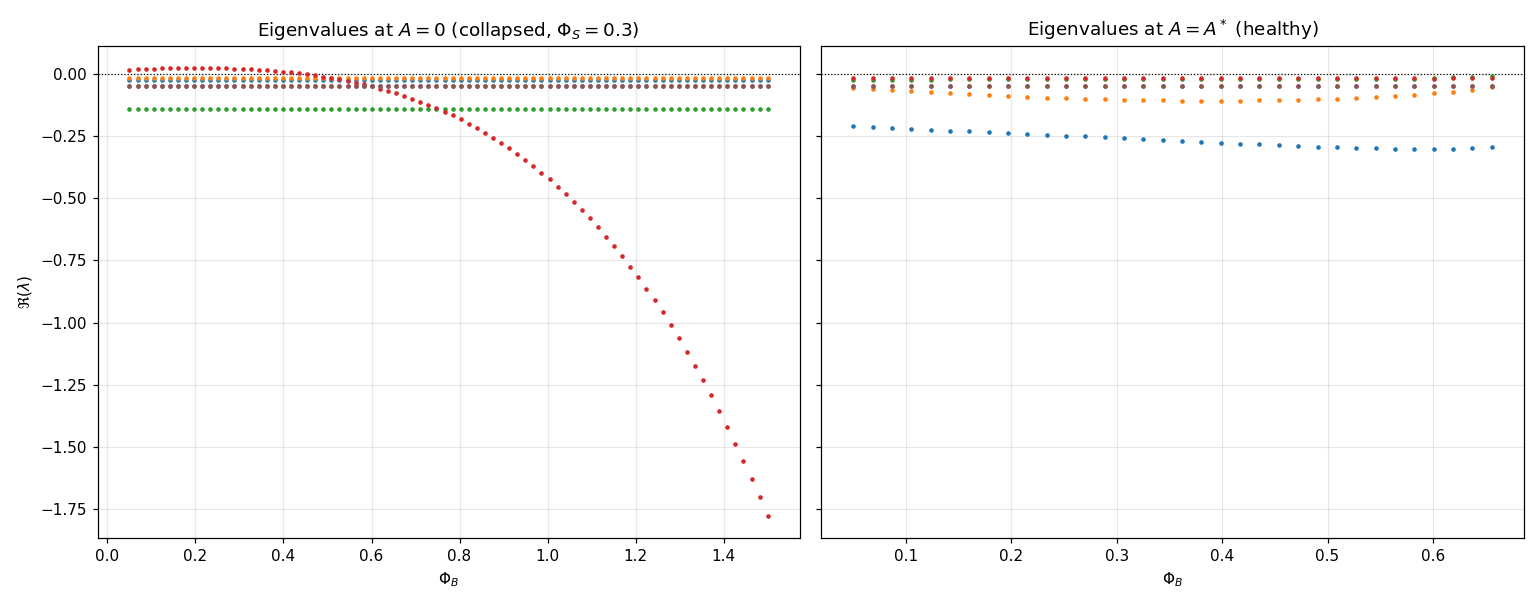
\includegraphics[width=\textwidth]{figures/v4_jacobian_eigenvalues.png}
    \caption{Real parts of the six Jacobian eigenvalues vs.\ $\Phi_B$ at $\Phi_S = 0.3$. (Left) at the boundary equilibrium $A=0$: five eigenvalues are constant (cascade rates), the sixth (the $A$-block) crosses zero at the transcritical bifurcation $\bar\mu(0;\Phi)=0$. (Right) at the healthy interior equilibrium $A=A^*$: all six eigenvalues are negative wherever $A^*$ exists.}
    \label{fig:v4_eigenvalues}
\end{figure}

\subsection{A Composite Lyapunov Function} \label{sec:v4-lyapunov}

Local stability is settled by the linearisation; for global descent toward the appropriate basin we construct a composite Lyapunov function exploiting the cascade.

\begin{theorem}[Composite Lyapunov decomposition]\label{thm:v4-lyap}
Let $V(y; \Phi) = V_K(y) + V_{BS}(y; A) + V_F(y; A) + V_A(A; \Phi)$ with the partial Lyapunov functions tabulated in Table \ref{tab:v4_lyapunov_summary}. There exist weights $w_K, w_B, w_S, w_F, w_A > 0$ and a constant $c > 0$, depending only on the model parameters and the regime, such that on every compact subset of the physical domain,
\[
\dot V \le -c\, V.
\]
Consequently, on a compact invariant region:
\begin{enumerate}
  \item In the mono-stable healthy regime, every initial condition converges exponentially to the unique interior equilibrium.
  \item In the bistable regime, every initial condition with $A_0 > A_{\rm sep}$ converges to the interior equilibrium $A^*$, and every initial condition with $A_0 < A_{\rm sep}$ converges to $A=0$.
  \item In the mono-stable collapsed regime, every initial condition converges to $A=0$.
\end{enumerate}
\end{theorem}

\begin{table}[h]
    \centering
    \begin{tabular}{lll}
\toprule
Block & Lyapunov component & Decay rate \\
\midrule
$K$-block      & $V_K = \tfrac{1}{2}\sum_i (K_{Fi}-K_{Fi}^*)^2$ & $1/\tau_K$ \\
$B$-block      & $V_B = \tfrac{1}{2}(B-B^*(A))^2$               & $1/\tau_B$ \\
$S$-block      & $V_S = \tfrac{1}{2}(S-S^*(A))^2$               & $1/\tau_S$ \\
$F$-block      & $V_F = \tfrac{1}{2}(F-F^*(A))^2$               & $a_F(A)/\tau_F$ \\
$A$-block (collapsed)  & $V_A = \tfrac{1}{2}A^2$                & $|\bar\mu(0;\Phi)|$ for $\bar\mu(0)<0$ \\
$A$-block (healthy)    & $V_A = \tfrac{\eta}{4}(A^2-(A^*)^2)^2$ & $2\eta(A^*)^2$ near $A^*$ \\
\bottomrule
\end{tabular}
    \caption{Per-block components of the composite Lyapunov function $V = V_K + V_B + V_S + V_F + V_A$. The decay rate of each block depends on a uniformly bounded coupling state ($A$ for $V_F$); cross-coupling is absorbed via Young's inequality with weights $w_*$ chosen so that $\dot V \le -c V$ globally on compact sets.}
    \label{tab:v4_lyapunov_summary}
\end{table}

\paragraph{Proof sketch.}
The $K$-block has decoupled linear dynamics, so $\dot V_K = -(2/\tau_K) V_K$ exactly. For the $(B, S)$ block at fixed $A$, $\dot V_B \le -(2/\tau_B) V_B + \alpha_B \|A - A^*\|$, where $\alpha_B$ is a Lipschitz constant of the autonomic-factor $a_B(A)$; an analogous bound holds for $V_S$. For the $F$ block, $\dot V_F \le -(2 a_F^{\min}/\tau_F) V_F + \alpha_F (\|A - A^*\| + \|K - K^*\|)$ where $a_F^{\min} > 0$ is bounded below on any compact $A$-set. For the $A$ block:
\begin{itemize}
  \item In the collapsed regime, $V_A = \tfrac12 A^2$ gives $\dot V_A = (\bar\mu(A) - \eta A^2) A^2 \le \bar\mu(0;\Phi) A^2 + \mathcal{O}(A^3) < 0$ for small $A$, with strict negativity uniform on compacts.
  \item In the healthy or bistable regime around an interior $A^*$, $V_A = \tfrac{\eta}{4}(A^2 - (A^*)^2)^2$ is a positive-definite double-well potential whose minima coincide with the stable equilibria; standard La Salle arguments confirm convergence within each basin.
\end{itemize}
The cross-coupling errors $\alpha_B \|A-A^*\|$, $\alpha_F \|K - K^*\|$, etc., are absorbed by Young's inequality $|xy| \le \tfrac12 \epsilon x^2 + \tfrac{1}{2\epsilon} y^2$ with $\epsilon$ chosen so the resulting block weights remain positive. The cascade structure guarantees that this can always be done, because each block's intrinsic decay rate is bounded below away from zero on the compact domain.\hfill$\square$

The full algebra (Young weights, regime-dependent decay constant $c$) is straightforward but tedious; we defer it to the appendix.

\subsection{Numerical Basin Diagrams} \label{sec:v4-basins}

The analytical separatrix $A_{\rm sep}(\Phi)$ is the basin boundary in the $A$-direction. Figures \ref{fig:v4_basin_phiB} and \ref{fig:v4_basin_phiS} show the basin classification in the $(\Phi_X, A_0)$ slice for $X \in \{B, S\}$ with the other stimulus fixed at $0.3$, computed by RK4 integration of \texttt{drift\_jax} (no diffusion) for 120 days. The analytical separatrix (dashed) and stable interior equilibrium (solid) match the numerical basin boundary to grid resolution.

\begin{figure}[h]
    \centering
    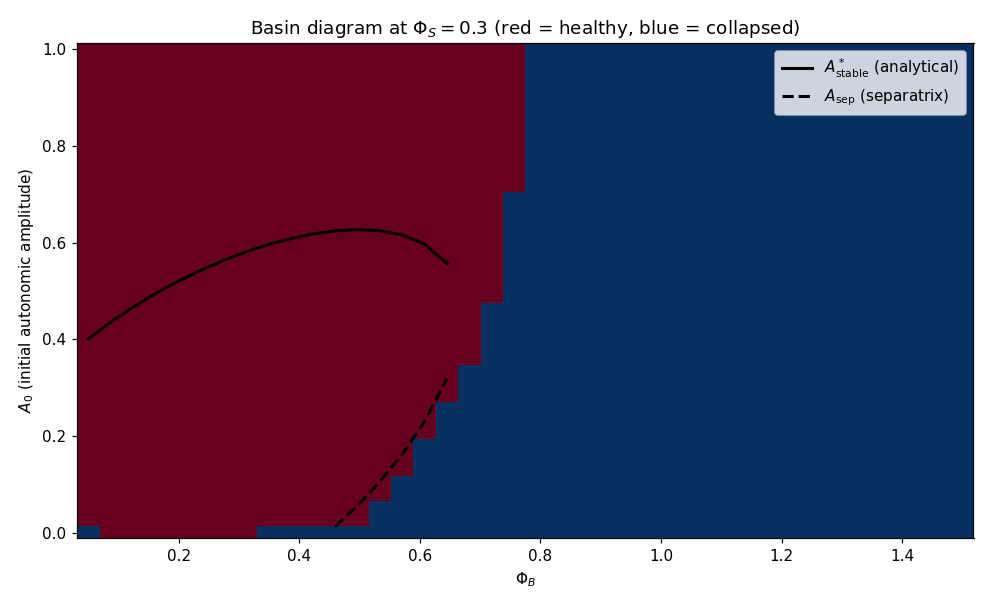
\includegraphics[width=0.85\textwidth]{figures/v4_basin_diagram_phiB.png}
    \caption{Basin classification at $\Phi_S = 0.3$. The bistable strip $\Phi_B \in [0.45, 0.75]$ exhibits two attractors: trajectories starting above the dashed separatrix $A_{\rm sep}$ rise to the solid stable curve $A^*_{\rm stable}$; trajectories starting below collapse. To the left of the transcritical (small $\Phi_B$), $A=0$ is unstable so even $A_0 \to 0^+$ rises. To the right of the saddle-node ($\Phi_B \gtrsim 0.75$), no interior equilibrium exists.}
    \label{fig:v4_basin_phiB}
\end{figure}

\begin{figure}[h]
    \centering
    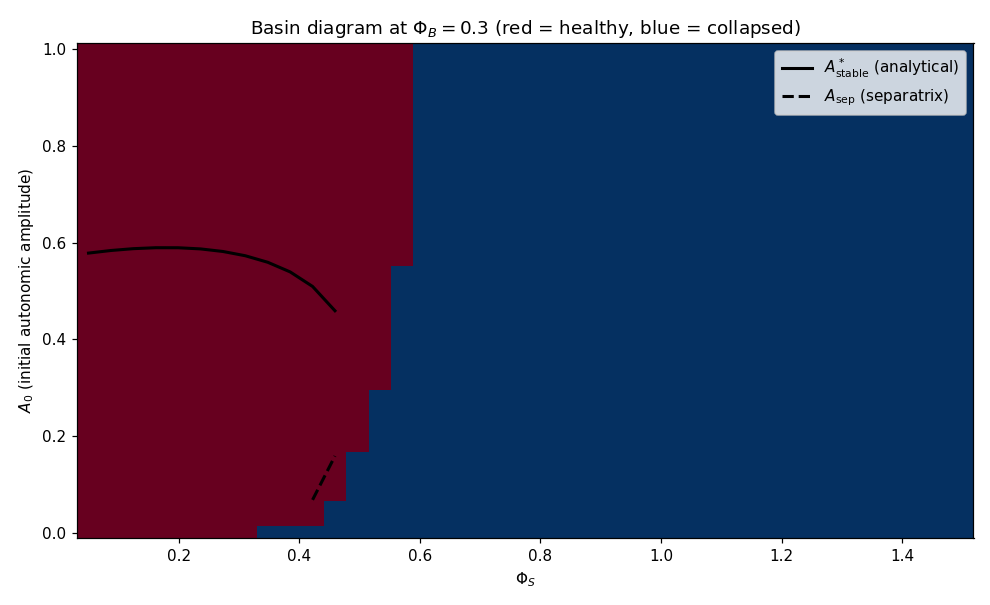
\includegraphics[width=0.85\textwidth]{figures/v4_basin_diagram_phiS.png}
    \caption{Symmetric slice: basin classification at $\Phi_B = 0.3$. The strength axis exhibits the same three-regime structure with a slightly different bifurcation location, because the $S$ system has weaker autonomic feedback ($\epsilon_{AS} < \epsilon_{AB}$) but faster fatigue gain ($K_{FS}^0 > K_{FB}^0$).}
    \label{fig:v4_basin_phiS}
\end{figure}

\subsection{Equilibrium Values} \label{sec:v4-eq-table}

Table \ref{tab:v4_equilibrium_values} reports the slow-manifold values $K^*, B^*, S^*, F^*$ and the autonomic equilibrium $A^*$ at a 5\,$\times$\,5 grid in $(\Phi_B, \Phi_S)$. ``$A^* = 0$'' means no positive interior root exists at that stimulus.

\begin{table}[h]
    \centering
    \scriptsize
    \begin{tabular}{cc|cccccc}
\toprule
$\Phi_B$ & $\Phi_S$ & $K_{FB}^*$ & $K_{FS}^*$ & $B^*$ & $S^*$ & $F^*$ & $A^*$ \\
\midrule
0.20 & 0.20 & 0.0510 & 0.0710 & 0.122 & 0.106 & 0.112 & $0.531$ \\
0.20 & 0.40 & 0.0510 & 0.0920 & 0.120 & 0.210 & 0.223 & $0.476$ \\
0.20 & 0.55 & 0.0510 & 0.1078 & 0.101 & 0.264 & 0.486 & $0$ \\
0.20 & 0.70 & 0.0510 & 0.1235 & 0.101 & 0.336 & 0.677 & $0$ \\
0.20 & 1.00 & 0.0510 & 0.1550 & 0.101 & 0.480 & 1.156 & $0$ \\
0.40 & 0.20 & 0.0720 & 0.0710 & 0.253 & 0.108 & 0.184 & $0.632$ \\
0.40 & 0.40 & 0.0720 & 0.0920 & 0.246 & 0.213 & 0.295 & $0.554$ \\
0.40 & 0.55 & 0.0720 & 0.1078 & 0.202 & 0.264 & 0.616 & $0$ \\
0.40 & 0.70 & 0.0720 & 0.1235 & 0.202 & 0.336 & 0.807 & $0$ \\
0.40 & 1.00 & 0.0720 & 0.1550 & 0.202 & 0.480 & 1.287 & $0$ \\
0.55 & 0.20 & 0.0877 & 0.0710 & 0.351 & 0.109 & 0.263 & $0.661$ \\
0.55 & 0.40 & 0.0877 & 0.0920 & 0.329 & 0.210 & 0.405 & $0.470$ \\
0.55 & 0.55 & 0.0877 & 0.1078 & 0.277 & 0.264 & 0.753 & $0$ \\
0.55 & 0.70 & 0.0877 & 0.1235 & 0.277 & 0.336 & 0.943 & $0$ \\
0.55 & 1.00 & 0.0877 & 0.1550 & 0.277 & 0.480 & 1.423 & $0$ \\
0.70 & 0.20 & 0.1035 & 0.0710 & 0.437 & 0.108 & 0.379 & $0.600$ \\
0.70 & 0.40 & 0.1035 & 0.0920 & 0.353 & 0.192 & 0.765 & $0$ \\
0.70 & 0.55 & 0.1035 & 0.1078 & 0.353 & 0.264 & 0.922 & $0$ \\
0.70 & 0.70 & 0.1035 & 0.1235 & 0.353 & 0.336 & 1.112 & $0$ \\
0.70 & 1.00 & 0.1035 & 0.1550 & 0.353 & 0.480 & 1.592 & $0$ \\
1.00 & 0.20 & 0.1350 & 0.0710 & 0.504 & 0.096 & 1.044 & $0$ \\
1.00 & 0.40 & 0.1350 & 0.0920 & 0.504 & 0.192 & 1.203 & $0$ \\
1.00 & 0.55 & 0.1350 & 0.1078 & 0.504 & 0.264 & 1.360 & $0$ \\
1.00 & 0.70 & 0.1350 & 0.1235 & 0.504 & 0.336 & 1.550 & $0$ \\
1.00 & 1.00 & 0.1350 & 0.1550 & 0.504 & 0.480 & 2.030 & $0$ \\
\bottomrule
\end{tabular}
    \caption{Slow-manifold equilibrium values across $(\Phi_B, \Phi_S) \in \{0.20, 0.40, 0.55, 0.70, 1.00\}^2$. Computed in closed form from \eqref{eq:K-star}--\eqref{eq:F-star} and root-finding for $A^*$. Each row satisfies $f(y^*; \Phi) = 0$ to machine precision (verified numerically; max $\|f\| < 10^{-14}$).}
    \label{tab:v4_equilibrium_values}
\end{table}

\subsection{Stochastic Extension (Provisional)} \label{sec:v4-stochastic}

The above analysis is for the deterministic flow. For the FSA-v4 SDE with state-dependent diffusion $\sigma(y)$, the same composite $V$ together with the Foster--Lyapunov inequality of Section \ref{sec:stability} extends to the 6D case via the generator
\[
\mathcal{L} V = \langle \nabla V, f \rangle + \tfrac12 \mathrm{tr}\big(\sigma \sigma^\top \nabla^2 V\big) \le -c V + c',
\]
with the noise contribution bounded by $c' = \tfrac12 \sigma_{\max}^2 \, \mathrm{tr}(\nabla^2 V)$ on compact sets. This proves geometric ergodicity to a unique stationary distribution within each basin, but does not on its own resolve metastable transition rates between basins --- the latter would require a Freidlin--Wentzell large-deviations analysis, which is beyond the scope of these notes.

\paragraph{Practical implication for the controller.}
Section \ref{sec:open_loop_limitation} argued that the open-loop trajectory optimiser is structurally unable to exhibit the periodisation behaviour described in Section \ref{sec:fsa-v4}. The basin geometry now makes the gap precise: in the bistable regime the controller must keep the system above the separatrix $A_{\rm sep}(\Phi(t))$ at all times, which is a state-feedback constraint that an open-loop schedule cannot enforce against noise. The SMC$^2$-based controller of Section \ref{sec:smc2_vs_ot} addresses this directly because its chance-constraint formulation can encode $\Pr[A_t < A_{\rm sep}(\Phi_t)] \le \alpha$ as a particle-rejection rule.
